\documentclass[11pt]{article} 
\usepackage{mathtools}
\usepackage[letterpaper, width=14cm, height=22cm, top=5cm]{geometry}       
 \headsep=1pt
\usepackage[parfill]{parskip}    % Activate to begin paragraphs with an empty line rather than an indent
\usepackage{graphicx}
\graphicspath{{./Images/}}
\usepackage{amssymb}
\usepackage{epstopdf}
\usepackage[usenames,dvipsnames]{color}
\usepackage{hyperref}
\hypersetup{colorlinks, urlcolor=Cyan, citecolor=Cyan, hyperfootnotes=false}
\usepackage[none]{hyphenat}

\usepackage{cite}
\setlength{\voffset}{-2cm}
\addtolength{\textheight}{2cm}
\addtolength{\textwidth}{3cm}
\addtolength{\hoffset}{-1.5cm}
\usepackage{fancyhdr}
\hyphenchar\font=-1

\begin{document}
C. S. Gorham\\
\today

\emph{SUMMARY OF varied time-step Kinetic Monte Carlo Simulation (KMCS):} Events, and the apparent time that it takes to complete the event, occur based on 1. how likely it is that they occur in a system of possible events, 2. a randomly generated number. 

1) KMCS\_coadsorb.py is a KMCS modeling the co-adsorption of  particles A and B, available in abundance, on a square lattice of finite size. The following are situations for which the simulation is run. The results are depicted through the figures herein and are described briefly. Further, the applicable .csv files are indicated and attached. 

{\bf{Figure 1 - Different Lattice sizes; All transition coefficients equal}}\\
\hspace*{1cm}It is clear from the results that restricting the number of sites that contribute to the event probability below a certain size leads to size effects characterized by increased noise, i.e., increased signal fluctuation from equilibrium results, and greater apparent time between events which is an artifact of the simulation. Thus, when conducting a KMCS it is important to ensure that the experimental system is large enough to avoid size effects. 


{\bf{ Figure 2 - Smaller transition coefficients; All transition coefficients equal }} \\
\hspace*{1cm}When the transition coefficients are relatively small, events are able to occur more often as less energy is required for the event. Thus, there is shorter time between events and equilibrium is reached after a shorter amount of time. The system also exhibits a smaller temperature dependence due to the fact that the activation energy in the numerator of the exponential factor dominates the exponent.


{\bf{Figure 3 - Larger transition coefficients; All transition coefficients equal}}\\
\hspace*{1cm}When the transition coefficients are relatively large, less events are able to occur because a greater amount of energy is required for the event to occur. Thus, there is longer time between events and equilibrium is reached after a longer amount of time. The system also exhibits a much larger temperature dependence due to the fact that the activation energy in the numerator of the exponential factor dominates the exponent.


{\bf{Figure 4 - absorb activation energy 2x}}\\
When the activation energy for absorption events is twice as large as that for desorption events, desorption events are much more likely to occur. Thus, the total coverage of the system is low. As desorption events can only occur after an absorption event has occurred, the number of events at lower temperatures is extremely small  - there appear to be no events during the simulation time for the system at 101 K, i.e., no particles absorb due to the high activation energy. 


{\bf{Figure 5 - desorb activation energy 2x}}\\
When the activation energy for desorption events is twice as large as that for absorption events, absorption events are much more likely to occur while these particles are unlikely to desorb. Thus, the total coverage of the system is high. \\

{\bf{Figure 6 - B activation energy 2x}}\\
When the activation energy  events of a particular family of particles is twice as large as that for all other events, all events for the other families of particles are much more likely to occur. Thus, the coverage of the family of particles with high activation energies exhibits a slower build-up and eventually surpasses that of the other families of particles (because it requires more energy to desorb). The event probability of other families of particles are un-affected, until the system reaches a saturation point where the build-up of the high activation energy family restricts the absorption of other families.

{\bf{Figure 7 - B-absorb activation energy 2x }}\\
When the activation energy for absorption events of a particular family of particles is twice as large as that for all other events, all other events are much more likely to occur. Thus, the coverage of that family of particles on the system is low, while the other type is unaffected. As desorption events can only occur after an absorption event has occurred, the number of events at lower temperatures is extremely small  - there appear to be no events during the simulation time for the system at 101 K, i.e., no particles absorb due to the high activation energy. 


{\bf{Figure 8 - B-desorb activation energy 2x }}\\
When the activation energy for desorption events of a particular family of particles is twice as large as that for all other events, all other events are much more likely to occur. Thus, the coverage of that family of particles on the system is high, while the other type is unaffected. 







\setlength{\unitlength}{1in}
\begin{figure}[h!]
\begin{tabular}{cc}
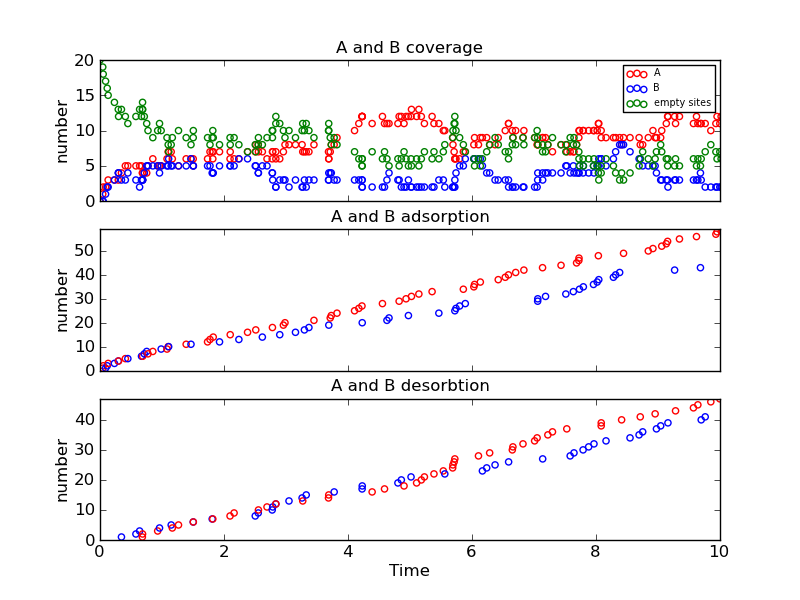
\includegraphics[width=3.5in, height=4.2in]{./coadsorb/AtoBcoadsorb2x10_301_allsamek__A5_EA5E3_1.png} &
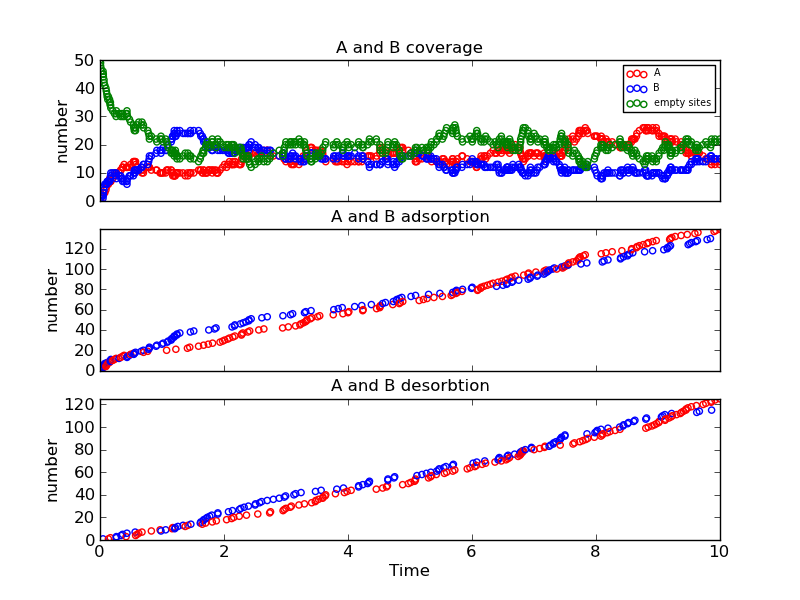
\includegraphics[width=3.5in, height=4.2in]{./coadsorb/AtoBcoadsorb5x10_301_allsamek__A5_EA5E3_1.png} \\
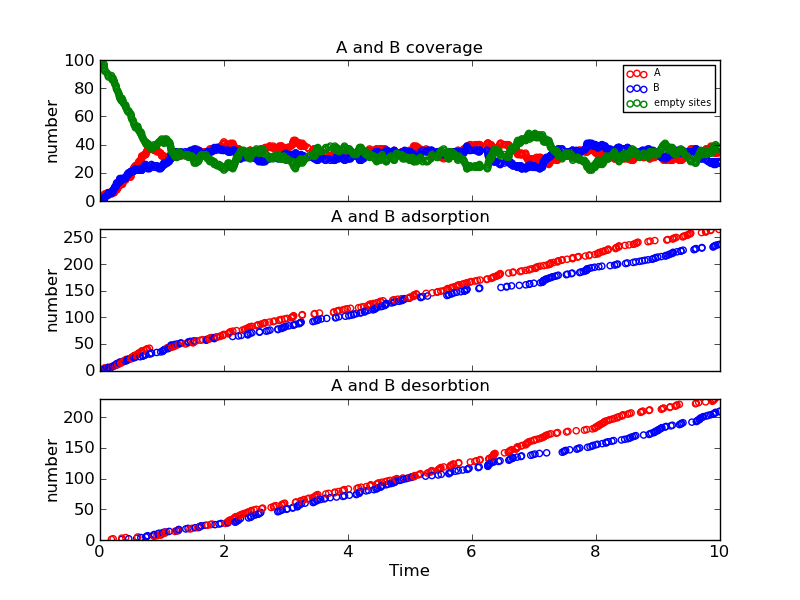
\includegraphics[width=3.5in, height=4.2in]{./coadsorb/AtoBcoadsorb10x10_301_allsamek__A5_EA5E3_1.png} &
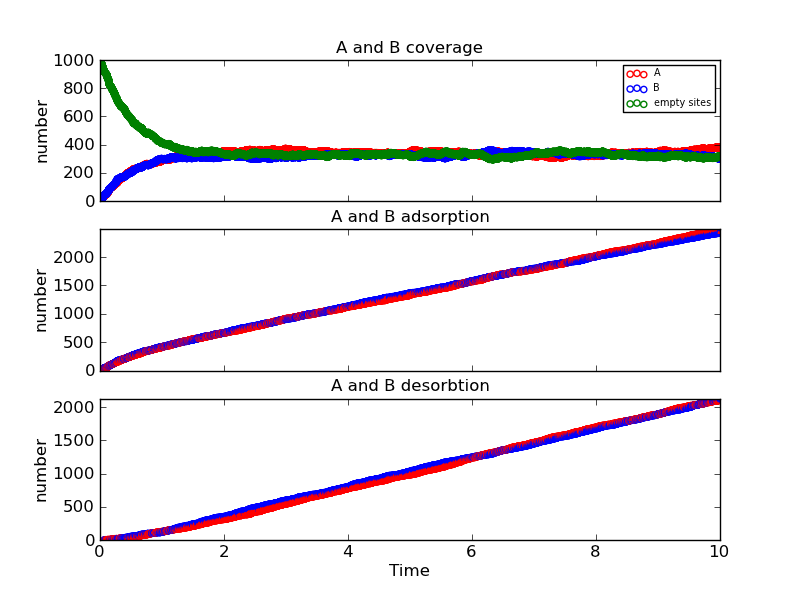
\includegraphics[width=3.5in, height=4.2in]{./coadsorb/AtoBcoadsorb100x10_301_allsamek__A5_EA5E3_1.png} 
\end{tabular}
\caption{The figures depict the effect (top of three:) total coverage of the systems simulated, (middle of three:) absorption of the particles present, (bottom of three:) and desorption of the particles present using different lattice sizes in the KMCS, where the transition coefficients do not depend on the position of the lattice. All simulations are run at 301K. In these simulations, all events have the same transition coefficient, where the activation energy is E$_a$=5kJmol$^{-1}$. [From top left to bottom right:] 2x10, 5x10, 10x10, 100x10. }
\end{figure}

\setlength{\unitlength}{1in}
\begin{figure}[h!]
\begin{tabular}{cc}
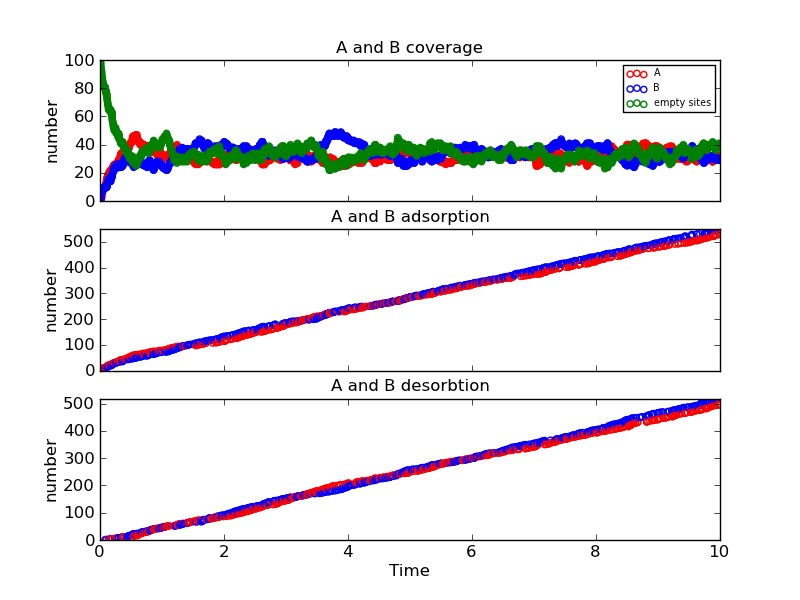
\includegraphics[width=3.5in, height=4.2in]{./coadsorb/AtoBcoadsorb10x10_101_allsameksmall__A5_EA1E3_1.png} &
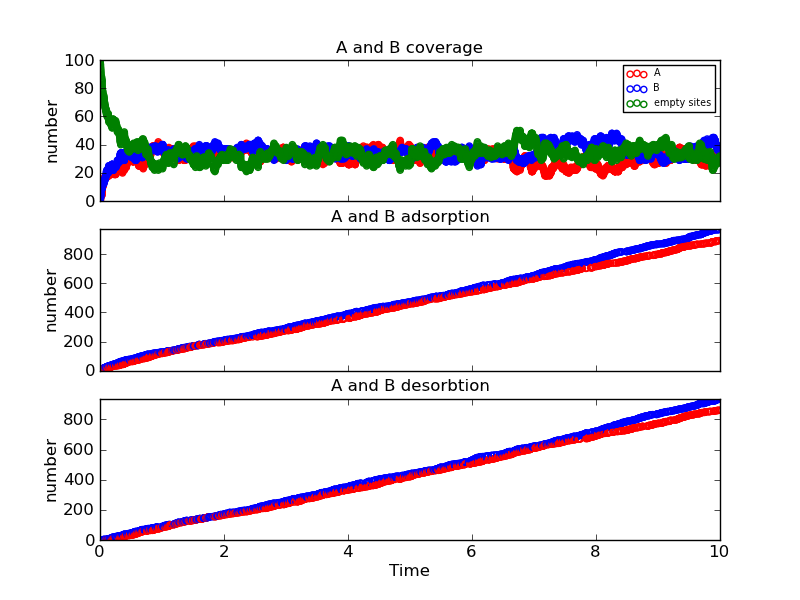
\includegraphics[width=3.5in, height=4.2in]{./coadsorb/AtoBcoadsorb10x10_201_allsameksmall__A5_EA1E3_1.png} \\
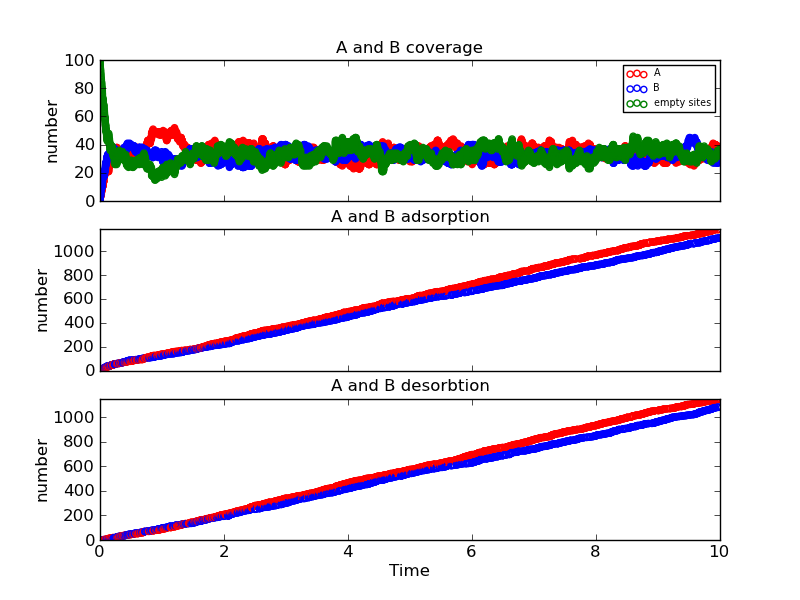
\includegraphics[width=3.5in, height=4.2in]{./coadsorb/AtoBcoadsorb10x10_301_allsameksmall__A5_EA1E3_1.png} &
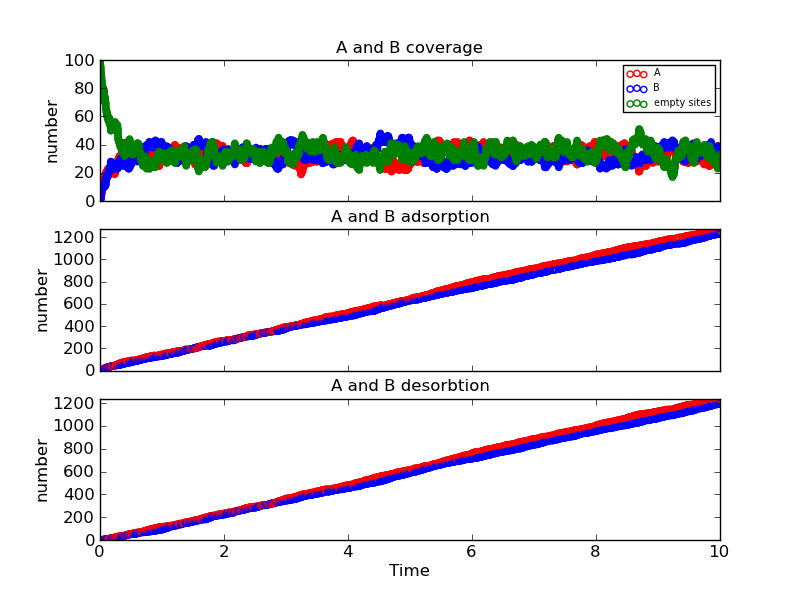
\includegraphics[width=3.5in, height=4.2in]{./coadsorb/AtoBcoadsorb10x10_401_allsameksmall__A5_EA1E3_1.png} 
\end{tabular}
\caption{This figure describes the (top of three:) total coverage of the systems simulated, (middle of three:) absorption of the particles present, (bottom of three:) and desorption of the particles present on a 10x10 lattice, where the transition coefficients to not depend on the position of the lattice. In these simulations, all events have the same transition coefficient, where the activation energy is E$_a$=1kJmol$^{-1}$. [From top left to bottom right:] 101 K, 201 K, 301 K, 401 K. }
\end{figure}

\setlength{\unitlength}{1in}
\begin{figure}[h!]
\begin{tabular}{cc}
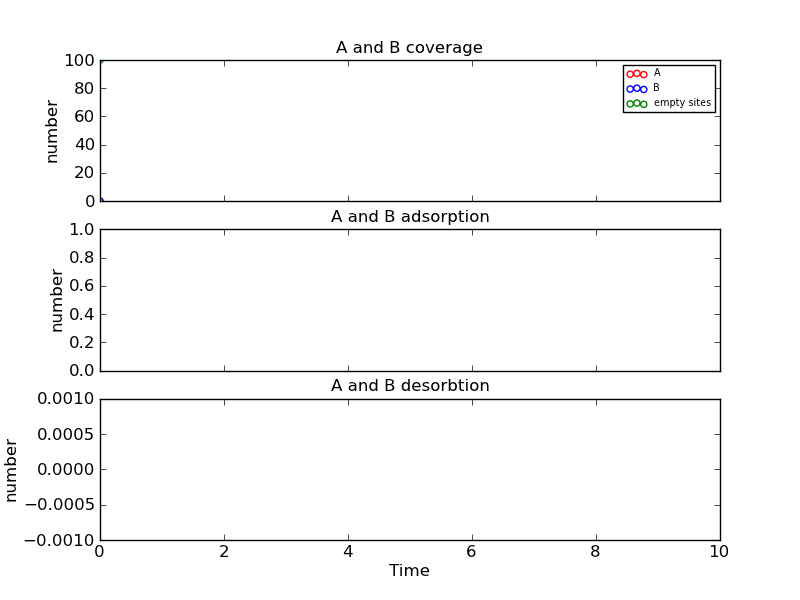
\includegraphics[width=3.5in, height=4.2in]{./coadsorb/AtoBcoadsorb10x10_101_allsameklarge__A5_EA10E3_1.png} &
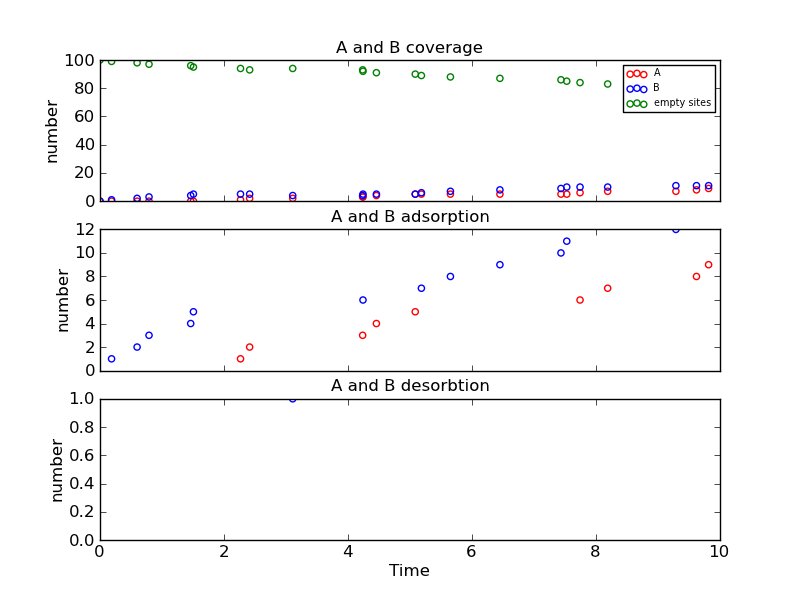
\includegraphics[width=3.5in, height=4.2in]{./coadsorb/AtoBcoadsorb10x10_201_allsameklarge__A5_EA10E3_1.png} \\
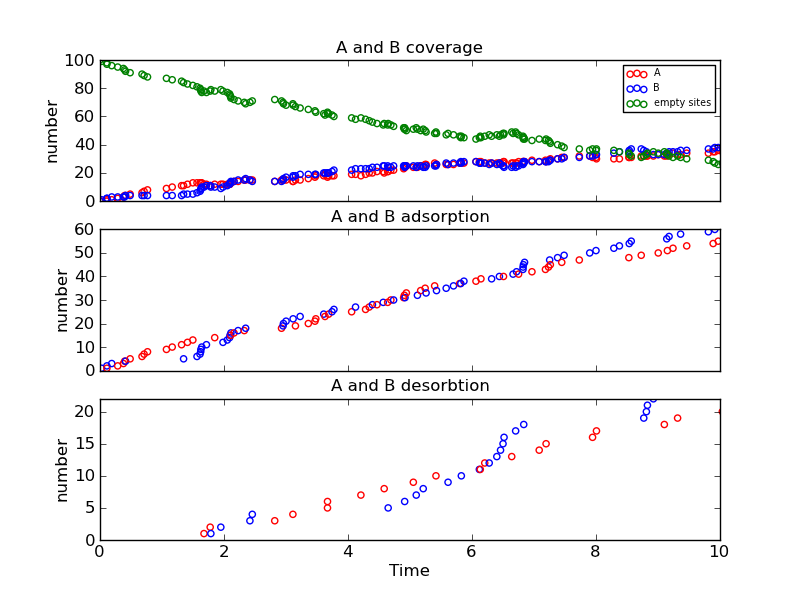
\includegraphics[width=3.5in, height=4.2in]{./coadsorb/AtoBcoadsorb10x10_301_allsameklarge__A5_EA10E3_1.png} &
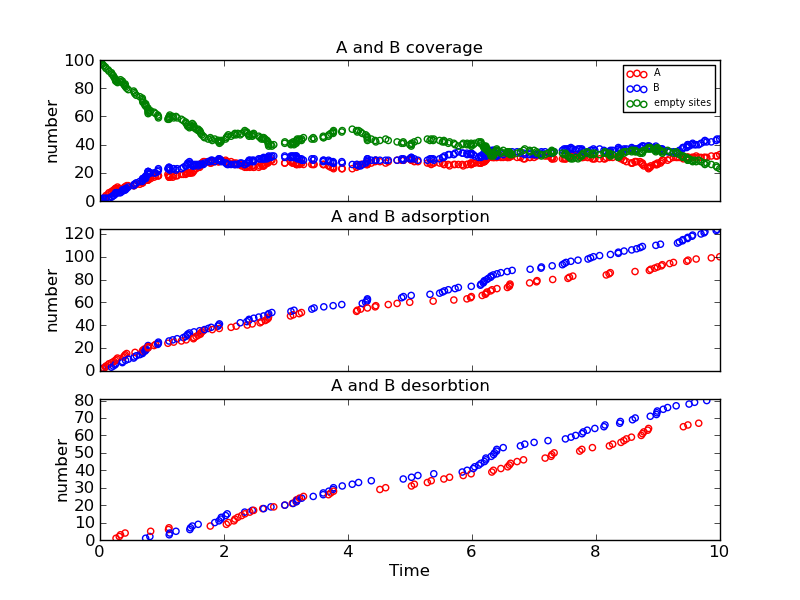
\includegraphics[width=3.5in, height=4.2in]{./coadsorb/AtoBcoadsorb10x10_401_allsameklarge__A5_EA10E3_1.png} 
\end{tabular}
\caption{This figure describes the (top of three:) total coverage of the systems simulated, (middle of three:) absorption of the particles present, (bottom of three:) and desorption of the particles present on a 10x10 lattice, where the transition coefficients to not depend on the position of the lattice. In these simulations, all events have the same transition coefficient, where the activation energy is E$_a$=10kJmol$^{-1}$. [From top left to bottom right:] 101 K, 201 K, 301 K, 401 K.. }
\end{figure}

\setlength{\unitlength}{1in}
\begin{figure}[h!]
\begin{tabular}{cc}
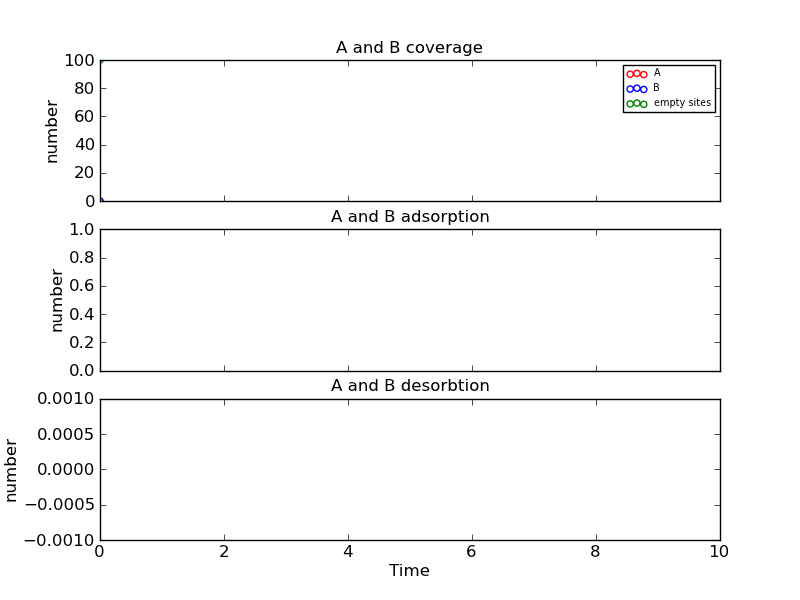
\includegraphics[width=3.5in, height=4.2in]{./coadsorb/AtoBcoadsorb10x10_101_absorb2x__Ea10E3_Ed5E3_1.png} &
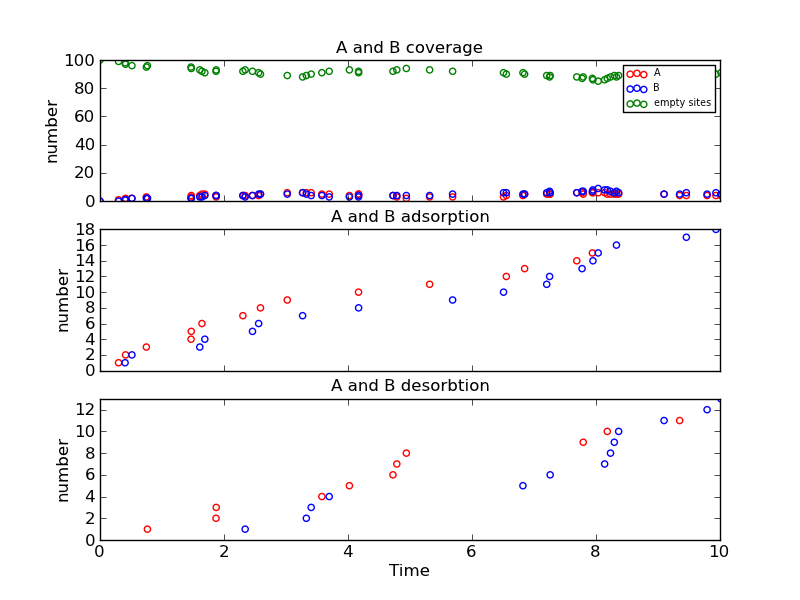
\includegraphics[width=3.5in, height=4.2in]{./coadsorb/AtoBcoadsorb10x10_201_absorb2x__Ea10E3_Ed5E3_1.png} \\
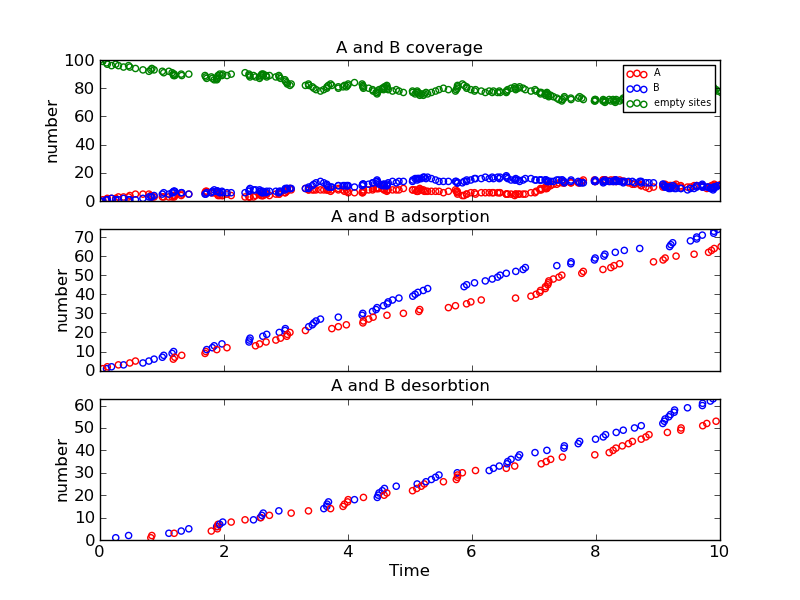
\includegraphics[width=3.5in, height=4.2in]{./coadsorb/AtoBcoadsorb10x10_301_absorb2x__Ea10E3_Ed5E3_1.png} &
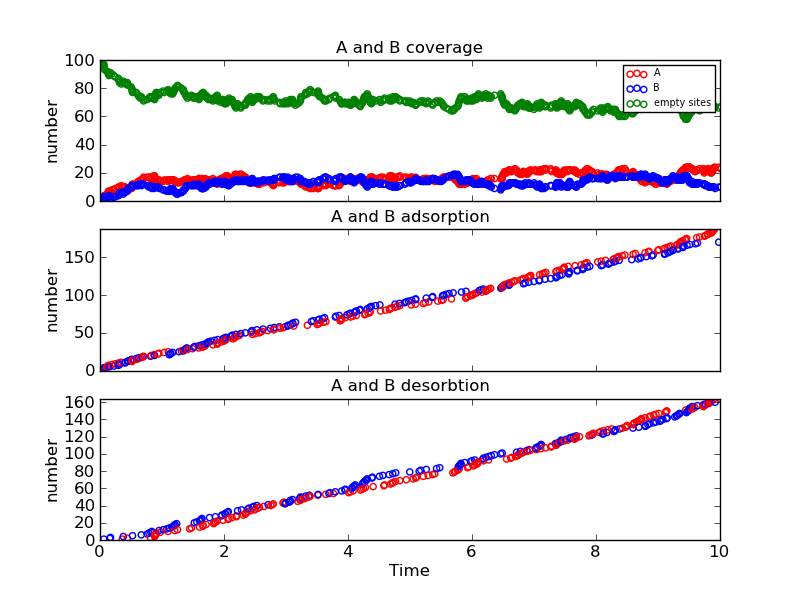
\includegraphics[width=3.5in, height=4.2in]{./coadsorb/AtoBcoadsorb10x10_401_absorb2x__Ea10E3_Ed5E3_1.png} 
\end{tabular}
\caption{This figure describes the (top of three:) total coverage of the systems simulated, (middle of three:) absorption of the particles present, (bottom of three:) and desorption of the particles present on a 10x10 lattice, where the transition coefficients to not depend on the position of the lattice. In these simulations, the activation energy of absorption of A and B is twice as large as that of desorption, where the activation energy is E$_{a_{absorption}}$=10kJmol$^{-1}$ and E$_{a_{desorption}}$=5kJmol$^{-1}$. [From top left to bottom right:] 101 K, 201 K, 301 K, 401 K. }
\end{figure}

\setlength{\unitlength}{1in}
\begin{figure}[h!]
\begin{tabular}{cc}
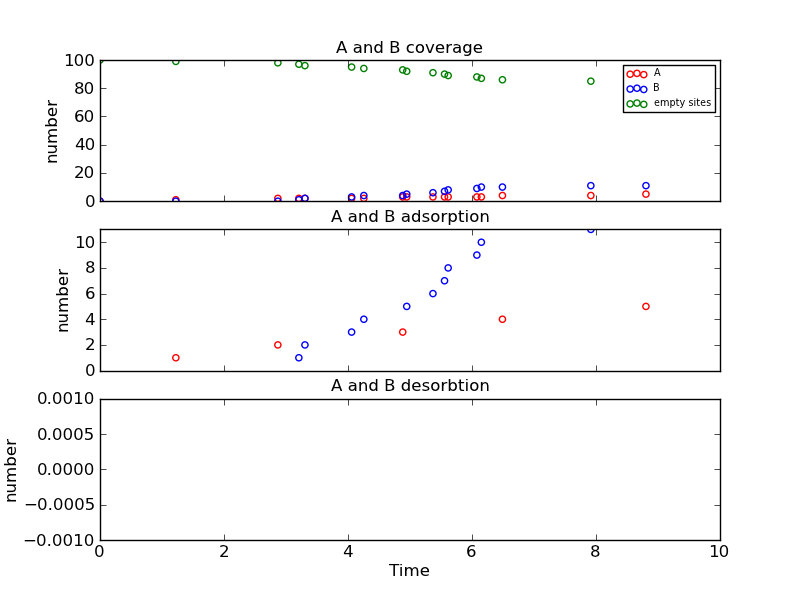
\includegraphics[width=3.5in, height=4.2in]{./coadsorb/AtoBcoadsorb10x10_101_desorb2x__Ea5E3_Ed10E3_1.png} &
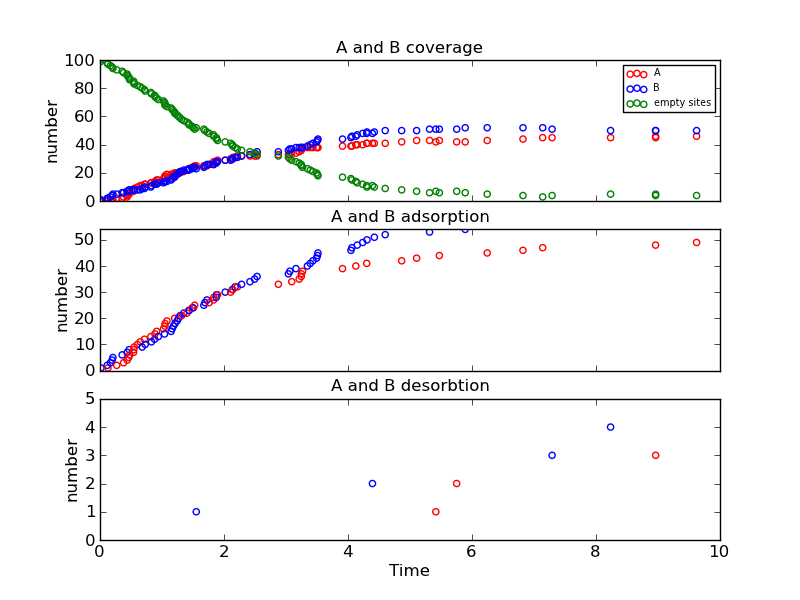
\includegraphics[width=3.5in, height=4.2in]{./coadsorb/AtoBcoadsorb10x10_201_desorb2x__Ea5E3_Ed10E3_1.png} \\
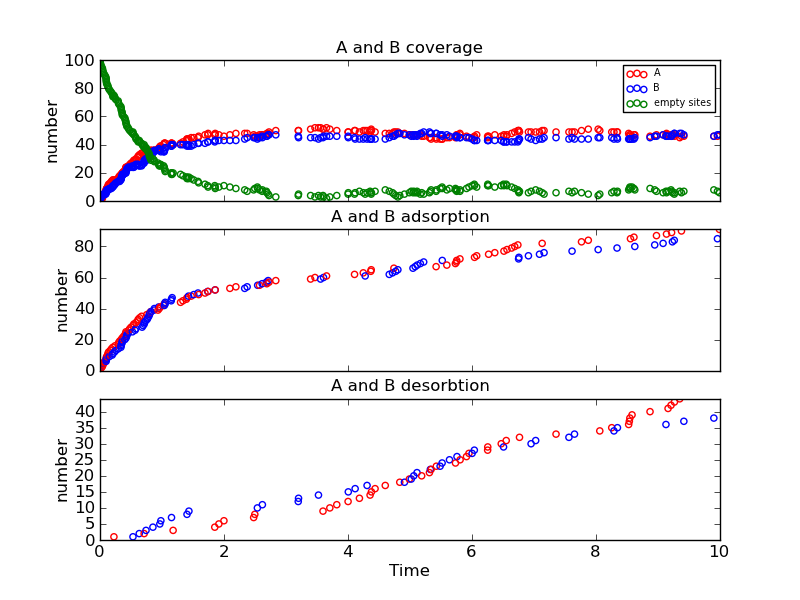
\includegraphics[width=3.5in, height=4.2in]{./coadsorb/AtoBcoadsorb10x10_301_desorb2x__Ea5E3_Ed10E3_1.png} &
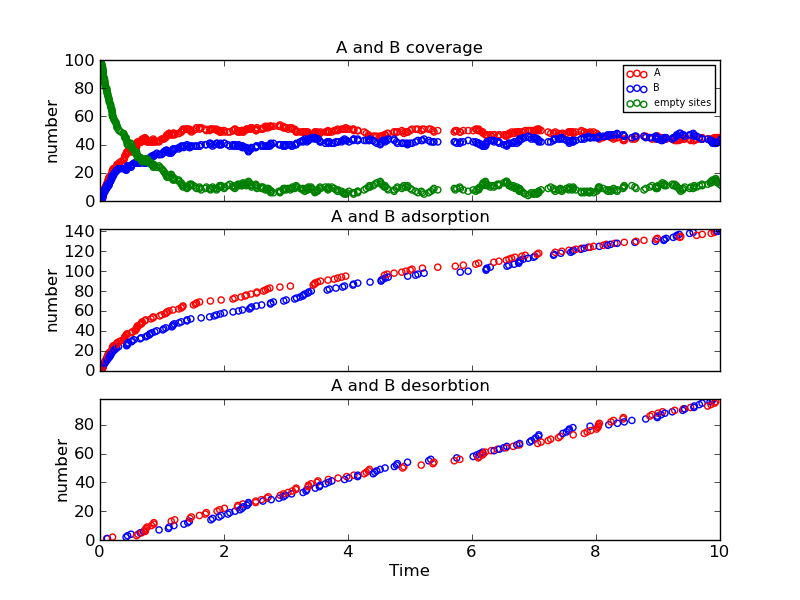
\includegraphics[width=3.5in, height=4.2in]{./coadsorb/AtoBcoadsorb10x10_401_desorb2x__Ea5E3_Ed10E3_1.png} 
\end{tabular}
\caption{This figure describes the (top of three:) total coverage of the systems simulated, (middle of three:) absorption of the particles present, (bottom of three:) and desorption of the particles present on a 10x10 lattice, where the transition coefficients to not depend on the position of the lattice. In these simulations, the activation energy of desorption of A and B is twice as large as that of absorption, where the activation energy is E$_{a_{desorption}}$=10kJmol$^{-1}$ and E$_{a_{absorption}}$=5kJmol$^{-1}$. [From top left to bottom right:] 101 K, 201 K, 301 K, 401 K. }
\end{figure}


\setlength{\unitlength}{1in}
\begin{figure}[h!]
\begin{tabular}{cc}
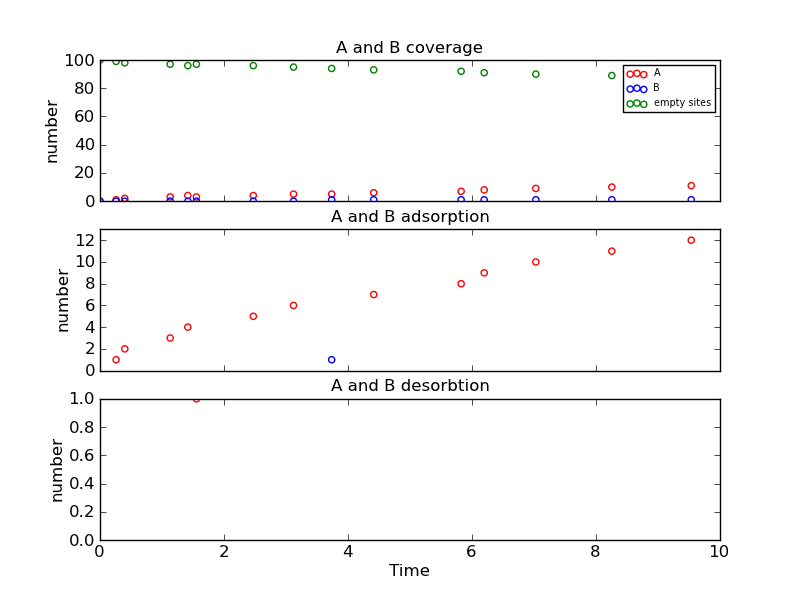
\includegraphics[width=3.5in, height=4.2in]{./coadsorb/AtoBcoadsorb10x10_101_B2x__EA5E3_EB10E3_1.png} &
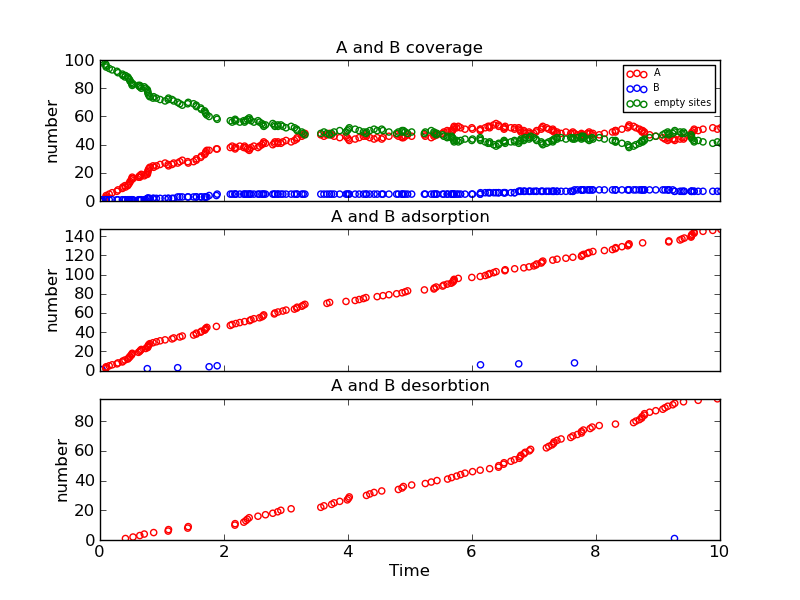
\includegraphics[width=3.5in, height=4.2in]{./coadsorb/AtoBcoadsorb10x10_201_B2x__EA5E3_EB10E3_1.png} \\
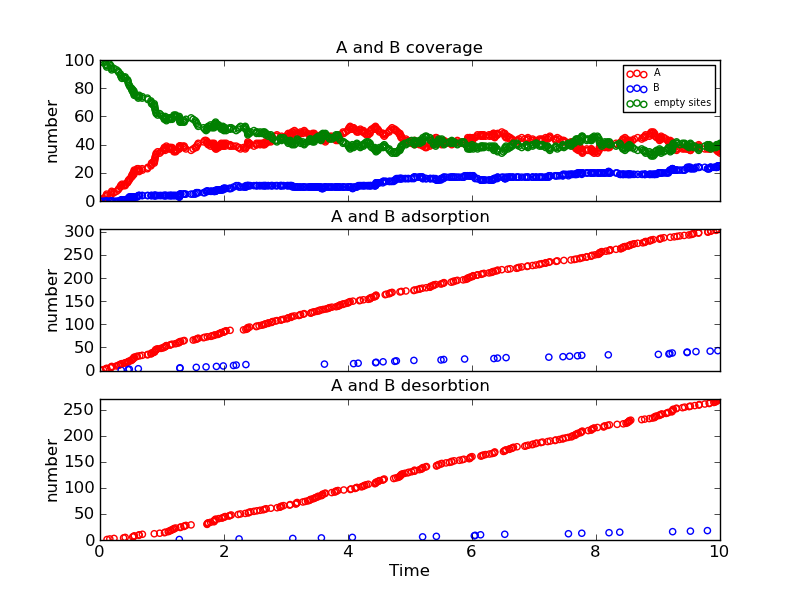
\includegraphics[width=3.5in, height=4.2in]{./coadsorb/AtoBcoadsorb10x10_301_B2x__EA5E3_EB10E3_1.png} &
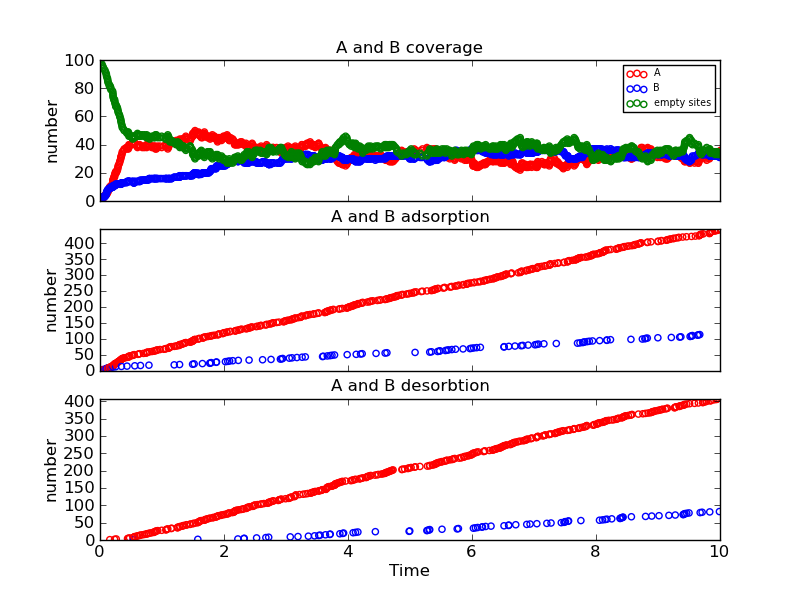
\includegraphics[width=3.5in, height=4.2in]{./coadsorb/AtoBcoadsorb10x10_401_B2x__EA5E3_EB10E3_1.png} 
\end{tabular}
\caption{This figure describes the (top of three:) total coverage of the systems simulated, (middle of three:) absorption of the particles present, (bottom of three:) and desorption of the particles present on a 10x10 lattice, where the transition coefficients to not depend on the position of the lattice. In these simulations, the activation energy associated with events involving B are twice as large as that of events involving A, where the activation energy is E$_{a_{B}}$=10kJmol$^{-1}$ and E$_{a_{A}}$=5kJmol$^{-1}$. [From top left to bottom right:] 101 K, 201 K, 301 K, 401 K.}
\end{figure}

\setlength{\unitlength}{1in}
\begin{figure}[h!]
\begin{tabular}{cc}
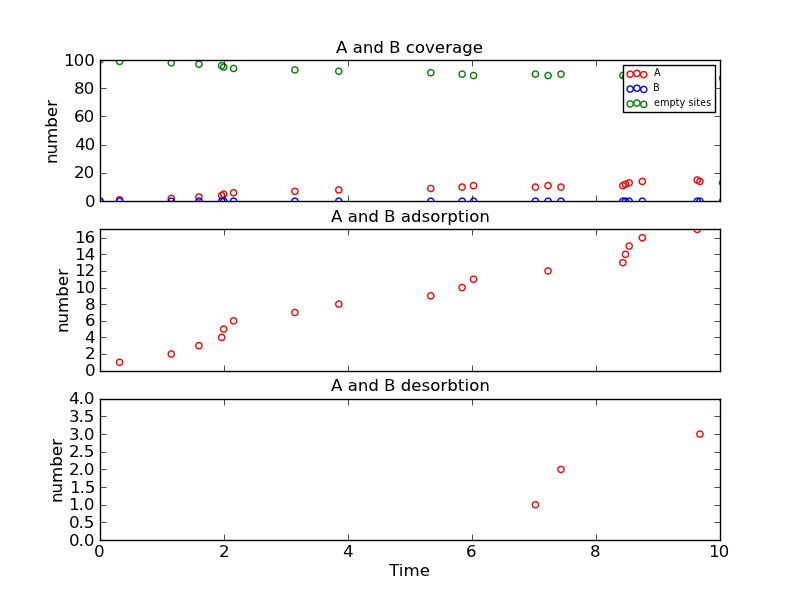
\includegraphics[width=3.5in, height=4.2in]{./coadsorb/AtoBcoadsorb10x10_101_Babs2x__EA5E3_EB10E3_1.png} &
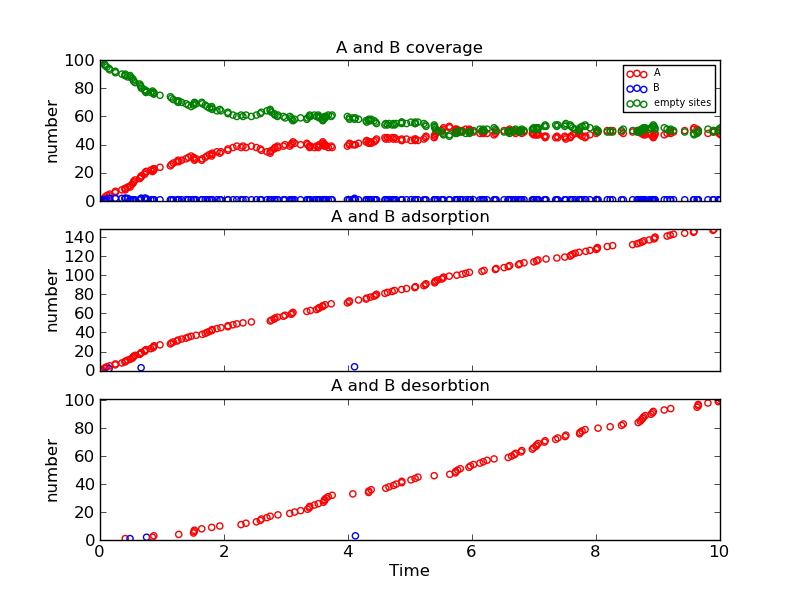
\includegraphics[width=3.5in, height=4.2in]{./coadsorb/AtoBcoadsorb10x10_201_Babs2x__EA5E3_EB10E3_1.png} \\
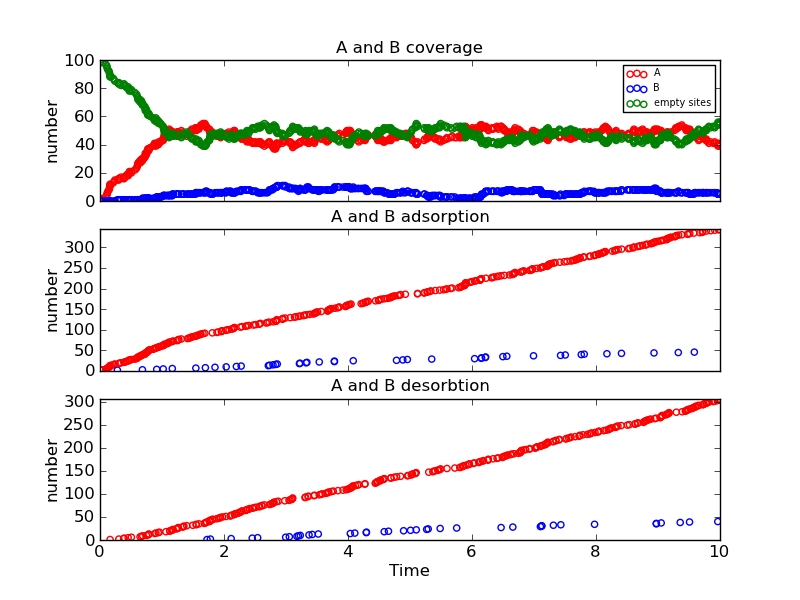
\includegraphics[width=3.5in, height=4.2in]{./coadsorb/AtoBcoadsorb10x10_301_Babs2x__EA5E3_EB10E3_1.png} &
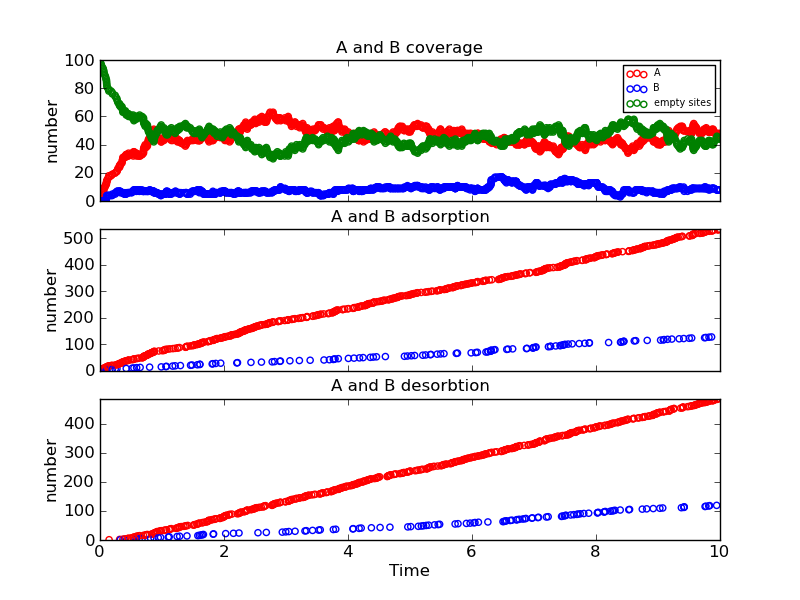
\includegraphics[width=3.5in, height=4.2in]{./coadsorb/AtoBcoadsorb10x10_401_Babs2x__EA5E3_EB10E3_1.png} 
\end{tabular}
\caption{This figure describes the (top of three:) total coverage of the systems simulated, (middle of three:) absorption of the particles present, (bottom of three:) and desorption of the particles present on a 10x10 lattice, where the transition coefficients to not depend on the position of the lattice. In these simulations, the activation energy associated with absorption events of B are twice as large as that of all other events, where the activation energy is E$_{a_{B:absorb}}$=10kJmol$^{-1}$ and E$_{a_{other}}$=5kJmol$^{-1}$. [From top left to bottom right:] 101 K, 201 K, 301 K, 401 K. }
\end{figure}

\setlength{\unitlength}{1in}
\begin{figure}[h!]
\begin{tabular}{cc}
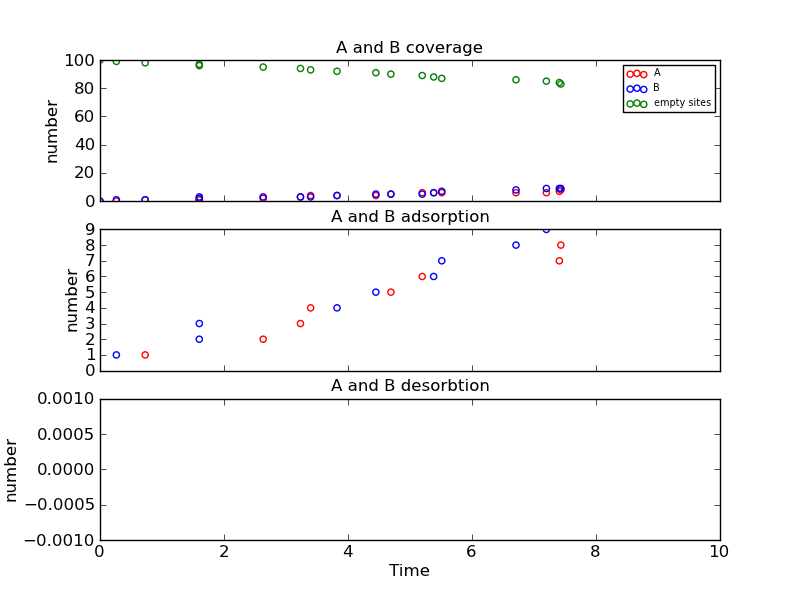
\includegraphics[width=3.5in, height=4.2in]{./coadsorb/AtoBcoadsorb10x10_101_Bdes2x__EA5E3_EBx10E3_1.png} &
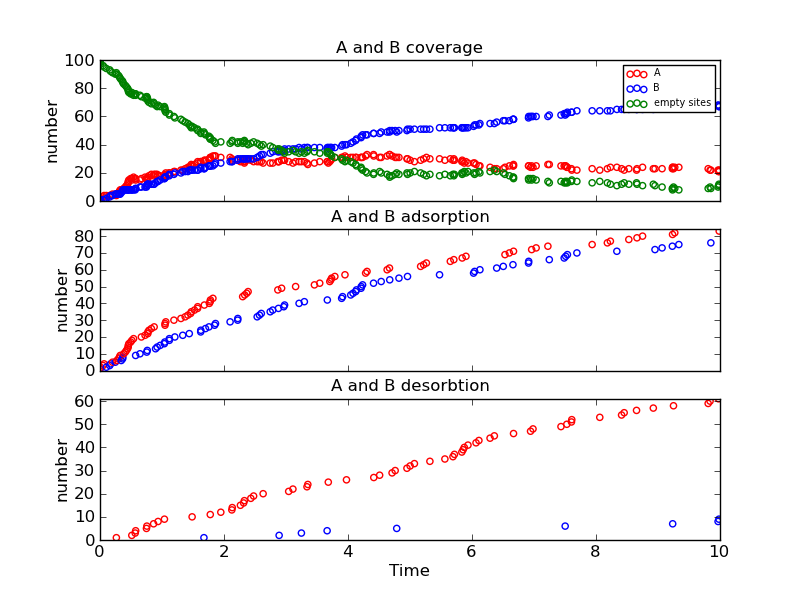
\includegraphics[width=3.5in, height=4.2in]{./coadsorb/AtoBcoadsorb10x10_201_Bdes2x__EA5E3_EBx10E3_1.png} \\
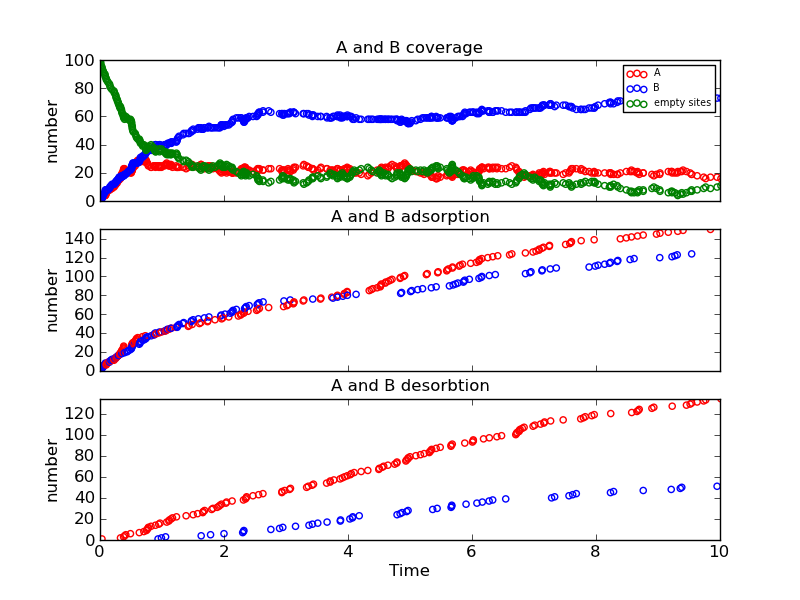
\includegraphics[width=3.5in, height=4.2in]{./coadsorb/AtoBcoadsorb10x10_301_Bdes2x__EA5E3_EBx10E3_1.png} &
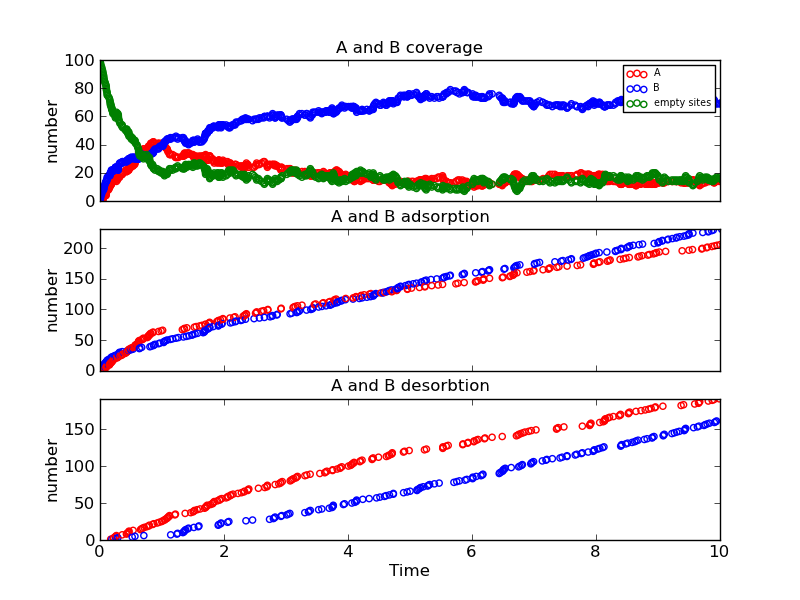
\includegraphics[width=3.5in, height=4.2in]{./coadsorb/AtoBcoadsorb10x10_401_Bdes2x__EA5E3_EBx10E3_1.png} 
\end{tabular}
\caption{This figure describes the (top of three:) total coverage of the systems simulated, (middle of three:) absorption of the particles present, (bottom of three:) and desorption of the particles present on a 10x10 lattice, where the transition coefficients to not depend on the position of the lattice. In these simulations, the activation energy associated with desorption events of B are twice as large as that of all other events, where the activation energy is E$_{a_{B:desorb}}$=10kJmol$^{-1}$ and E$_{a_{other}}$=5kJmol$^{-1}$. [From top left to bottom right:] 101 K, 201 K, 301 K, 401 K.}
\end{figure}

\end{document}